
% Cal Poly Thesis
% 
% based on UC Thesis format
%
% modified by Mark Barry 2/07.
%

\documentclass[12pt]{ucthesis}
\usepackage{ifpdf}

\newif\ifpdf
\ifx\pdfoutput\undefined
    \pdffalse % we are not running PDFLaTeX
\else
\pdfoutput=1 % we are running PDFLaTeX
\pdftrue \fi

\usepackage{url}
\usepackage{multicol}
\usepackage{cite}

\ifpdf
    \usepackage[pdftex]{graphicx}
    % Update title and author below...
    \usepackage[pdftex,plainpages=false,breaklinks=true,colorlinks=true,urlcolor=blue,citecolor=blue,
		linkcolor=blue,bookmarks=true,bookmarksopen=true,%
		bookmarksopenlevel=3,pdfstartview=FitV,
		pdfauthor={Kevin Schapansky},
		pdftitle={Jester: A Device Abstraction and Data Fusion API for Skeletal Tracking Sensors},
		pdfkeywords={thesis, masters, cal poly}]{hyperref}
    %Options with pdfstartview are FitV, FitB and FitH
    \pdfcompresslevel=1

\else
    \usepackage{graphicx}
\fi

\usepackage{hyperref}
\hypersetup{
	linktoc=all,
    colorlinks,
    citecolor=black,
    filecolor=black,
    linkcolor=black,
    urlcolor=black
}

\usepackage{titlesec}
% \titleformat{\chapter}[display]% OLD
%     {\normalfont\huge\bfseries}{\chaptertitlename\ \thechapter}{20pt}{\Huge}% OLD
% \titlespacing*{\chapter}{0pt}{50pt}{40pt}% OLD
\titleformat{\chapter}[display]% NEW
    {\normalfont\centering}{\chaptertitlename\ \thechapter}{12pt}{}% NEW
\titlespacing*{\chapter}{0pt}{30pt}{20pt}% NEW

%\titleformat{\section}[block]{first}{label}{12pt}

\titleformat{\section}{}{\thesection}{1em}{}
\titleformat{\subsection}{}{\thesubsection}{1em}{}
\titleformat{\subsubsection}{}{\thesubsubsection}{1em}{}
\titleformat{\paragraph}{}{\theparagraph}{1em}{}

\usepackage[font={}]{caption}

%\renewcommand{\cftchapleader}{\cftdotfill{\cftdotsep}} % for chapters
%\renewcommand{\cftsecleader}{\cftdotfill{\cftdotsep}} 


\usepackage{amssymb}
\usepackage{amsmath}
\usepackage[letterpaper,papersize={8.5in,11in}]{geometry}
\usepackage[overload]{textcase}
\usepackage[toc,page]{appendix}

\usepackage{tabularx}
\usepackage{algorithm}
\usepackage{algpseudocode}

\usepackage{enumitem}
\setlist{nolistsep}


\floatstyle{boxed}
\restylefloat{table}

%\bibliographystyle{abbrv}

\setlength{\parindent}{0.25in} \setlength{\parskip}{6pt}

\geometry{verbose,nohead,tmargin=1in,bmargin=1in,lmargin=1.5in,rmargin=1in}

\setcounter{tocdepth}{3}
\setcounter{secnumdepth}{3}


% Different font in captions (single-spaced, bold) ------------
%\newcommand{\captionfonts}{\small\bf\ssp}
\newcommand{\captionfonts}{}

\makeatletter  % Allow the use of @ in command names
\long\def\@makecaption#1#2{%
  \vskip\abovecaptionskip
  \sbox\@tempboxa{{\captionfonts #1: #2}}%
  \ifdim \wd\@tempboxa >\hsize
    {\captionfonts #1: #2\par}
  \else
    \hbox to\hsize{\hfil\box\@tempboxa\hfil}%
  \fi
  \vskip\belowcaptionskip}
\makeatother   % Cancel the effect of \makeatletter
% ---------------------------------------

\begin{document}

% Declarations for Front Matter

% Update fields below!
\title{Jester: 
A Device Abstraction and Data Fusion API 
for Skeletal Tracking Sensors}
\author{Kevin Schapansky}
\degreemonth{June} \degreeyear{2014} \degree{Master of Science}
\defensemonth{June} \defenseyear{2014}
\numberofmembers{3} \chair{Professor Zo{\"e} Wood, Ph.D.,\newline Department of Computer Science} \othermemberA{Assistant Professor Chris Lupo, Ph.D.,\newline Department of Computer Science} \othermemberB{Professor Franz Kurfess, Ph.D.,\newline Department of Computer Science} \field{Computer Science} \campus{San Luis Obispo}
\copyrightyears{seven}

\maketitle

\begin{frontmatter}

% Custom made for Cal Poly (by Mark Barry, modified by Andrew Tsui).
\copyrightpage

% Custom made for Cal Poly (by Andrew Tsui).
\committeemembershippage

\begin{abstract}

Humans naturally interact with the world in three dimensions. Traditional personal computers have relied on 2D mice for input because 3D user tracking systems were cumbersome and expensive. Recently, 3D input hardware has become accurate and affordable enough to be marketed to average consumers and integrated into niche applications. Presently, 3D application developers must learn a different API for each device their software will support, and there is no simple way to integrate sensor data if the system has multiple 3D input devices. This thesis presents Jester, a library that aims to simplify the development and improve the accuracy of 3D input-supported applications by providing an easily-extensible set of sensor wrappers that abstract the hardware specific details of capturing skeletal data and fusing sensor data in multiple 3D input device systems. Jester is then successfully used to create a toy application that uses real time skeletal tracking and sensor fusion of data from a Leap Motion and a PrimeSense Carime.

\end{abstract}

\begin{acknowledgements}

Thanks to:

\begin{itemize}
\item My advisor Zo{\"e} Wood, for being literally the coolest.
\item My parents for money and love.
\end{itemize}

\end{acknowledgements}

\tableofcontents

\listoftables

\listoffigures

\end{frontmatter}

\pagestyle{plain}

\renewcommand{\baselinestretch}{1.66}

% ------------- Main chapters here --------------------

\chapter{Introduction}
Hardware mice have been the dominant way that humans interact with the digital world ever since the first personal computers that introduced the concept of interacting mainly with a two dimensional graphical user interface instead of a text based terminal. Computer mice are very simple to manufacture and are an effective tool for interacting with strictly two dimensional applications such as word processing or managing an email inbox because they are bound to two dimensional sensing surfaces like a table top or flat laptop trackpad. Traditional computer programs and operating systems are designed to follow the “Windows, Icons Menus, Pointer” (WIMP) computer interaction paradigm. WIMP attempts to make a good digital analogue for a physical desktop where documents and folders are essentially managed in two dimensions [citation needed].

Even though using a mouse for WIMP-style two dimensional applications is a fairly simple task that even small children master quickly, it quickly becomes a handicap when trying to manipulate 3D applications, games, or even general computer navigation tasks that do not necessarily conform to the WIMP style, such as switching workspaces or web browser tabs [citation needed]. Since humans live in a 3D world by default, the human body itself makes an excellent 3D input device, just like how a computer mouse bound to sensing a two dimensional table top makes an excellent two dimensional sensing device.

\section{Gesture HCI}

Humans live every day of their lives in a 3D world. Our bodies are 3D and every physical object with which we interact is 3D. This makes the human body, and generally the hands, a natural choice for interacting with computers in a more intuitive manner. For example, when a user first attempts to interact with 3D Computer Aided Design (CAD) software with a mouse, there is a steep learning curve before he can fluidly and correctly navigate through the world. Different mouse or keyboard buttons are generally used to differentiate between scaling, rotating, and translating the object that is being designed [citation needed]. Application specific key combinations are not innately intuitive, even if they do become second nature after extended use of the software.The user’s hands are a perfect input choice because they are the interface he has been using to interact with the world around him ever since he was able to correctly place a triangle shaped block in a triangle shaped hole. Tracking the users hand and finger position allows object manipulation in CAD software to become innately intuitive through the use of standard grabbing, rotating, and pushing or pulling gestures [citation needed].

Nintendo introduced the concept of games that are controlled by the human body to millions of users in 2006. The Nintendo Wii includes sensors that can detect the position of user’s hands and comes bundled with a simulated sports package that allows users to use their arms to intuitively play digital sports [citation needed]. In 2011, Microsoft brought marker-less gesture interaction to mainstream gaming with the introduction of the Kinect for Xbox [citation needed]. The Kinect uses a technology called structured light, which will be discussed in the next chapter, to track the position of a player’s entire body. Human body tracking allows the users to control the Xbox using arm movements without picking up a controller or even play a game that allows users to compete against each other in a virtual dance off [citation needed].

Gesture interaction has also been applied to tasks that do not have as clear of a mapping to real life as CAD or video games. For example, gestures can be used to easily switch between browser tabs or navigate web pages [citation needed]. Also, work is being done on creating 3D file browsers where users can “shuffle through” digital documents and spreadsheets just like they would with physical paper. The task of arranging and moving files between folders can also be intuitively modeled using grab, move, and drop gestures that simulate arranging physical objects [citation needed].

\section{The Human Skeleton}

In order to accurately track the position of a human’s body it is necessary to pick some form of conceptual model that can accurately represent it. Muscle and connective tissue systems are extremely complex, and would be very difficult to represent intuitively or with any reasonable accuracy. Eliminating muscles and tendons leaves the skeletal system as the only remaining option. The human skeleton is an excellent choice for representing body position since it is the frame to which every other part of the body attaches. It is not necessary to track all 206 bones in the body since many bones can be approximated as a single bone, such as the bones in the feet or spinal column, or, like the ribs, are simply not necessary to establish the position of a person. A simplified skeletal rigging system is frequently used in computer animation to recreate how muscle and skin move in response to changing skeletal position [citation needed]. The reduced skeleton is both conceptually simple and can be used to accurately represent body position. Most 3D input devices have associated APIs that provide data about either skeletal joints, which can be trivially used to infer bone position, or direct bone position.

\section{3D Input Devices}

Historically, 3D input systems have been cumbersome and very expensive. They required complex sensor systems that either mounted to the body, or relied on the user wearing a skinsuit covered in motion markers [citation needed]. There are also early version that use computer vision techniques, but they were notoriously inaccurate and sensitive to lighting and user clothing [citation needed]. The expense of setting up a sensor room or the hassle of wearable instrumentation essentially guaranteed that these systems were only used in academic research or high budget special effects.

Within the last two years, there has been an explosion of fairly accurate and consumer-affordable 3D input devices. In 2011 Microsoft unveiled the Kinect for the Xbox 360 [citation needed]. The Kinect is capable of fairly accurately tracking the user’s torso and limbs, but not finer details like fingers. Several other devices like the Leap Motion Controller, released in 2013,  and the Creative Senz3D, released in 2014, are capable of accurately tracking hands and fingers. Finger tracking sensors generally have a limited field of view and range so they cannot track a user’s entire body. There are also hardware-based sensors like the Razer Hydra or the Oculus Rift that are capable of tracking with very high precision and minimal setup time. Each of these sensors has its own unique API for querying skeletal data.

\section{3D Applications}

Many of the initial applications designed to take advantage of 3D input devices were games and targeted to be more entertaining than useful. There are several games for Xbox that use the Kinect to judge a user’s dancing skill [citation needed]. Several PC games have also been ported to use the Oculus Rift and Razer Hydra to provide a more immersive gaming experience [citation needed]. Some scientific visualization and CAD software has begun to support the Leap Motion Controller, but a majority of its applications are still games. There has been work on using the Leap Motion and other short range finger sensing devices to navigate desktop workspaces or web browsing, but it is mostly experimental. All of these applications only support a small subset of the sensors that could be used to accomplish the same level of control.

\section{Jester's Contribution}

The human body is a proven method for intuitively and accurately interacting with simulated 3D environments and new and affordable 3D input devices targeted at consumers are flooding the market. However, there is still a significant barrier preventing 3D applications from taking off. Developers must individually tailor their applications to support specific sensors. Also, since sensors that are good at tracking details can rarely see a user’s whole body and wide angle sensors cannot see enough detail to accurately track fingers, developers must custom craft a data fusion system if they want the best features of both sensors. Jester provides an easily extensible library that simplifies the process of creating an application that can use 3D input devices by providing a framework for creating thin-wrappers to map the skeletal data of any sensor into Jester’s internal model of the skeleton as well as a framework for filtering and fusing data from multiple sensors. Application designers only need to write a thin wrapper for their sensor of choice that maps positional data to any bone or joint that is being tracked. Their application the has access to a world space skeleton and effortlessly adapted to use any available 3D input device.

\chapter{Background}

Jester’s core function of providing a solid framework for passing data from a sensor to a skeletal model requires only an understanding of how 3D positions can be transformed into different coordinate spaces and how quaternions handle rotations. The peripheral technologies like ranging solutions and filtering algorithms also warrant explanation. These technologies will be briefly explained in the following subsections.

\section{Spatial Mathematics}

Jester stores its skeletal knowledge as a hierarchy of bones where each bone stores its position and orientation relative to its parent bone’s coordinate space. It also provides the ability to set bone positions from skeletal joint coordinates in arbitrary space. The design and implementation of the bone hierarchy and joint transforms will be discussed in section \ref{sec:bone_hierarchy}. Understanding sections \ref{sec:bone_hierarchy} will require a basic understanding of matrix spatial transforms and quaternions.

\subsection{Spatial Transforms}

The space of an object is the 3D extents within which other objects have relative position. In the cartesian style spaces used in Jester, each dimension of the space is specified by a 3D vector, or basis vector, that is defined in its parent space \cite{gortler2012foundations}. All of Jester’s basis vectors are orthonormal, meaning they are orthogonal and unit length. Orthonormal bases simplify the process of reasoning about skeletal positioning because they guarantee that all of the dimensions can be measured with the same units. Spaces do not have to be specified in this manner, but more complex spaces are unnecessary for this application and lie outside the scope of this thesis. 

Jester spaces are specified in the traditional 3D computer graphics style where a 4x4 matrix, also known as a transformation matrix, is used to define and represent the space. The transformation matrix is constructed by combining the x, y, and z basis vectors with a vector specifying the translation of the new space within its parent. The 4th row of the matrix holds a basis vector that allows the matrix to be used for affine transformation. The layout of the matrix is shown in \ref{fig:transformation_mat}. A 3D point specified in the new space can be converted, or transformed, into the corresponding 3D point in the parent space by multiplying the point by the transformation matrix of the new space. In order for the multiplication to be possible, a fourth dimension must be added to the point. The fourth dimension is known as the homogeneous component and allows points and vectors to be handled correctly \cite{roberts1963machine}. Similarly, a 3D point can be brought from the parent space to the child space by multiplying the point by the inverse of the child’s transformation matrix.

\subsection{Quaternions}

Quaternions are a complex mathematical construct that effectively stores a 3D axis and the amount of rotation around that axis. They are less intuitive, but they allow rotations to be combined without the possibility of the gimbal lock problem that can occur when specifying a rotation as an euler rotation which is a combination of separate cascading rotations about the x, y, and z axes. Gimbal lock occurs when rotation about one axis causes the other two axes to be on the same plane. If two axes are coplanar a degree of freedom has essentially been lost \cite{gortler2012foundations}. Figure \ref{fig:gimbal_lock} demonstrates how a 90 degree rotation about the z axis causes the y and x axes to both specify rotation about the y axis.

\section{Sensor Types}

There are many different sensors that have begun to become popular in the consumer 3D input device market. They can be broadly broken into two categories: devices that require the user to wear trackable markers or sensors, and devices that use some form of imaging technology to observe the scene. Both categories contain many sub-types. Some current commercial examples will be examined and broadly explained. Jester is capable of working with any sensor that can produce data about a joint’s or bone’s position and orientation. The process of using the sensor with Jester will be explained briefly below. More detail about the Jester API and its use can be found in section \ref{sec:sensor_wrappers}. 

\subsection{Wearable Sensors}

Wearable sensors require that either trackable objects or the actual sensor itself is placed on the body part that the user wishes to track. They have the advantage of being very resistant to interference from ambient light, and are generally more accurate than other approaches. The trade off is that there is more setup time involved to place sensors and each bone or joint requires a separate sensor or marker \cite{zhu2004real}. Figure \ref{fig:wearables} shows the wearable sensors that will be discussed in sections \ref{sec:sixense}, \ref{sec:oculus}, and \ref{sec:prio}. 

\subsubsection{Sixense STEM}\label{sec:sixense}

The Sixense STEM system can track up to 3 remote tags, STEM packs, and two handheld controllers in the x, y, and z dimensions as will the roll, pitch, and yaw, known as six degrees of freedom, using magnetic field sensors (6 DOF) \cite{sixense_stem}. Relying on magnetic field rather than some sort of visual sensor means that the STEM system is impervious to any sort of lighting or UV interference. Using the STEM system with Jester would be as simple as getting the controller and STEM pack data from the Sixense API, associating the data points with the correct Jester bones or joints, and calling the newData() function on the Jester Controller.

\subsubsection{Oculus Rift}\label{sec:oculus}

The Oculus Rift is primarily a head mounted display, but it accurately detects head orientation using gyroscopes in order to provide the ability to look around the virtual environment \cite{oculus2012oculus}. The orientation returned by the Oculus API could easily be assigned to the head bone and then fused with the head position given by some other sensor in the Jester data fusion framework to provide both head orientation and position with minimal overhead.

\subsubsection{PrioVR}\label{sec:prio}

Yeti Technology is set to start delivering the first units of its new PrioVR system in Fall of 2014. The PrioVR system provides a set of Inertial Measurement (IMU) sensors that are designed to be attached to all of the main extremities on the user. The sensors reconcile their positions against the position of the main sensor unit which is mounted near the sternum to establish the pose of the user \cite{priovr}. PrioVR is perfectly suited to send data to Jester since it already senses the position and orientation of all of the major bones that are tracked by Jester.

\subsection{Imaging Sensors}

Imaging sensors capture the light reflected off of the user in order to determine his position. Some emit their own light in order to simplify the process of ranging and others rely entirely on ambient light. Therefore, all of them are sensitive to ambient lighting conditions and can be rendered ineffective by either too much ambient light or, in the case of passive sensors, not enough \cite{besl1988active}. They do not require markers to be placed on the user and can be designed to have very minimal setup times. Some examples of imaging sensors and their consumer implementations are discussed below.

\subsubsection{2D Cameras}

Traditional 2D cameras can be used to gather skeletal data. Extensive research has been done in attempting to subtract irrelevant background from 2D images and isolate the desired features. However 2D imaging techniques remain very sensitive to differences in ambient light and background color or texture. Due to these limitations, 2D cameras are not frequently used in consumer 3D user input devices that expect and reasonable level of accuracy \cite{shimada2001real}.

\subsubsection{Structured Light}

Structured light sensors work by emitting a pattern of infrared light like the one shown in figure \ref{fig:carmine_light}. When the pattern strikes objects, it distorts based on the angle of the object and its distance to the sensor. The sensor has a camera that is designed to only respond to infrared light that senses how the emitted pattern is reflected off of the user. The sensor then internally maps the emitted pattern to the distorted pattern to figure out pattern’s transform. The transform gives the distance to that particular part of the image. The sensor combines all of the distances into a depth image where grayscale color corresponds to the distance to that particular pixel. If any ambient light source produces more infrared light than the emitter, structured light sensors lose accuracy very quickly \cite{scharstein2003high}.

The PrimeSense Carmine and the Kinect are both examples of structured light sensors. They have an effective range of approximately 1 to 3 meters and have supporting libraries that map the output depth image to an estimated model of the user’s joint positions. These joint positions can be fed directly into Jester and Jester will reconstruct the position of the skeletal bones using known mappings from joints to bones. The Jester example program presented in this thesis uses the PrimeSense Carmine and will be discussed in more detail in section \ref{sec:carmine_impl}.

\subsubsection{Time of Flight}

Time of flight sensors, at a high level, emit pulses of light and then measure how long the light takes to return to the sensor in order to estimate distance. They are much more accurate than structured light sensors and are less sensitive to ambient light because they are not attempting to interpret a pattern of light, just the existence of return pulses \cite{litime} Figure \ref{fig:tof} explains the ranging technique used in the Texas Instruments time of flight sensor. 

Time of flight is replacing structured light as the technology of choice for many depth cameras. Microsoft has switched to time of flight technology for the second version of the Kinect \cite{kinect2}. Intel has partnered with Creative to subsidize the Senz3D sensor in order to push gesture-based interaction more into the mainstream. Both the manufacturer of the camera, SoftKinetic, and Intel have APIs for the Senz3D that track fingers on a hand \cite{senz3d}. The finger tracking data can be attached to the Jester hand bones and sent into the Jester API.

\subsubsection{Stereo Cameras}

Stereo camera systems are, at their simplest level, two of the same model of camera mounted a known distance apart from each other. Depth can be estimated by capturing an image from both cameras simultaneously, finding the common elements in both images, and calculating the distance based on the known distance between the cameras and the difference in position of the common elements in the images. Generally speaking, a smaller difference means the objects are far away from the camera and a larger difference means that they are closer \cite{lucas1981iterative}. Stereo cameras can either rely on natural light, or be assisted by infrared LEDs. Assisted stereo cameras are more impervious to varying lighting conditions, so the stereo setups in the commercial market are generally assisted.

One well known assisted stereo camera is the LeapMotion Controller. The LeapMotion Controller uses two cameras augmented with three infrared LEDs and is placed on a desktop facing upwards at a user’s hands. It resolves the distance to the hands and attempts to pick out the user’s individual fingers \cite{weichert2013analysis}. The LeapMotion Controller has an API that can be queried for hand and finger position. The Jester usage example presented in this paper uses the Leap API and will be discussed in greater detail in section \ref{sec:leap_impl}.

\section{Filtering Algorithms}

Positional data that comes from any real world sensor is subject to some level of noise and inaccuracy. Filtering algorithms attempt to establish some sort of likelihood model for new sensor readings in order to “trust” good measurements more than bad measurements. This is particularly useful for skeletal tracking sensors because tracking errors can sometimes occur that cause the estimated position of bones to jump wildly and then return to a consistent track. Good filtering algorithms will not assign much weight to the jumping measurements and so the filtered skeleton will be much more stable. Two filters that are well documented and have a strong following are Kalman filters and particle filters. Jester supports filtering plugins and an example particle filter has been implemented

\subsection{Kalman Filter}

The Kalman filter was introduced by Rudolf Kalman in 1960 as a new solution to linear filtering and prediction. His filter observes how measurements of a linear system change over time and attempts to estimate the true state of the system. Kalman filters operate using an update loop that for each iteration takes the current state of the system, uses a linear estimator function to guess how the system will change between measurements, corrects the estimation using the next sensor measurement, and sets the current system state to the corrected estimation \cite{kalman1960new}. 

The closer that the measurement is to the estimated state the more effect it will have on the system state. Measurement error is assumed to be gaussian, which means that readings should be strongly grouped around the actual true state. Kalman filters heavily rely on the accuracy of the estimation function which means that the quality of the filter requires that there is an accurate linear method for solving the system dynamics. For example, a Kalman filter would be an excellent choice for tracking the position of a vehicle using GPS. It is trivial to estimate how the position of a vehicle changes if the speed and direction are known, and GPS measurements are usually centered around the ground truth unless the satellite signal is extremely weak and so can be assumed to be Gaussian. 

A Kalman filter would be a suboptimal choice for filtering skeletal data. There is not a good equation for modeling skeletal position dynamics because human extremities can change speed and direction fairly rapidly. Limb movements rarely stay constant for more than a short period of time because humans have limited range of motion. 

\subsection{Particle Filter}

Particle filters are designed to filter systems where the estimation function is either nonlinear of extremely complex. They use a population of discrete guesses about the state of the system. Each guess is represented by one particle. When a particle filter is created the particles all contain uniformly selected random system states. Upon each sensor reading each particle is mutated either randomly or through some change heuristic and then is given a weight based on the gaussian probability of the particle’s guess given the sensor reading. A new set of particles is generated by selecting, with replacement, from the existing particle set in a manner that gives particles with higher probabilities a greater chance of being sampled. The new set of particles replaces the old set. The filter determines the estimated true state of the system by sampling the particle set in some manner that assumes the true measurement lies within the highest density of particles. Even though the filter is created with random guesses, the mutation and resampling process will cause the particles to cluster into groups that represent the best guesses at the state of the system \cite{sanjeev2002tutorial}. 

A particle filter is a good choice for skeletal tracking because it does not require any more than a basic heuristic guess about how the system is changing between samples and still provides filtering performance that is comparable to Kalman filters. However, particle filters are much more computationally expensive than Kalman filters so tradeoffs must be made between accuracy, by varying the particle count, and the need for real-time performance. A sample particle filter has been implemented and is discussed in detail in section \ref{sec:filter_impl}.

\chapter{Related Works}

Jester is similar to several existing frameworks for abstracting different parts of the skeletal data input process. Most of the research in this area to date has been focused on either a lower or higher level of abstraction and does not provide the flexibility that is built into Jester

\section{OpenNI}

OpenNI is a nonprofit organization focused on abstracting the process of retrieving depth, standard RGB, or audio data from sensors. Their API is designed to work with third party middleware in order to provide analysis and processing functionality to a wide range of sensors with minimal overhead. The project is open source and allows developers to write wrappers for their sensor drivers to port data into OpenNI’s input framework. The OpenNI API allows developers to have a single point of access for operations like detecting if devices are connected to the system or starting and stopping data streams. Providing developers with a single interface for communicating with sensors greatly simplifies the development process because the problems associated with supporting and compiling against multiple APIs are eliminated. It also benefits hardware manufacturers by making it easier for developers to adopt new sensors.

A majority of the hardware that are supported by the OpenNI API is manufactured by the companies that formed the partnership that founded OpenNI. There are some community written sensor wrappers, but they can be difficult to locate because there is no central repository. PrimeSense, the major driving force behind the OpenNI project, was purchased by Apple in November of 2013 and is no longer providing active support. The main web portal for downloading OpenNI and middleware binaries has been taken down. There is a GitHub repository for the OpenNI source, but it is no longer maintained.

\section{The Point Cloud Library}

The Point Cloud Library (PCL) is a large scale open source project for processing point cloud data. Point clouds are a method for representing range data where each each range measurement is stored as a 3D point in space. These points resemble clouds when visualized in 3D. The PCL has extensive support for data filtering, feature detection, registering clouds between frames to determine movement, and surfacing. It also has input modules that accept a large variety of depth sensors. Essentially any sensor that outputs 3D depth information can be adapted to work with the PCL \cite{rusu20113d}.

The PCL is used heavily by industry and research and is integrated with many open source and proprietary projects. It is an excellent tool for creating software that can manipulate the raw depth data from sensors and would be a good choice for writing an API that can estimate skeletal position using any depth sensor. The PCL’s abstraction of sensor input using point clouds in order to build a sophisticated higher level feature set is precisely what Jester is trying to achieve for taking bone position data and providing a framework to easily fuse and filter data into a consistent skeleton model for easy manipulation.

\section{Vrui Toolkit}

The Vrui Toolkit is an open source development toolkit that allows VR application developers to be shielded from the input and output configuration details of a virtual environment. Vrui supports display abstraction by creating OpenGL contexts that can be assigned to any combination of monitors or head mounted displays as well as a library of 3D UI widgets that allow developers to create 3D interfaces in the same manner as traditional 2D GUI editors. Input is abstracted with “semantic events” that notify the application about interaction events and input from a set of input tools like 3D pointers or 2D mice. It also provides a framework for splitting the input and output abstractions onto remote systems to allow parallelism and remote operation. Vrui is designed to provide a full suite of common VR functionality with dependencies that have excellent cross operating system support in order to maximize system compatibility \cite{kreylos2008environment}. 

Vrui attempts to tackle the VR abstraction problem with a monolithic software architecture that can handle the entire stack from hardware data capture to output. This massive software stack makes it difficult to change the functionality of any sub unit without side effects. It is also difficult to use the Vrui input abstraction without the rest of the system which arbitrarily increases the complexity of attempting to process the sensor driven input events in a different manner than the intended design. These constraints are not necessarily a problem for 3D applications that follow more of a 2D input paradigm, but it does limit flexibility. Vrui also does not have any support for fusing input data from separate sources.

\section{MiddleVR}

MiddleVR is closed source middleware that is designed to simplify the creation and deployment of VR applications. It is designed, like Vrui, to handle all aspects of building a VR application. It has an extensive supported input and output devices list that allows developers to seamlessly use a wide variety of devices. MiddleVR can use the Unity framework for output. Unity is an existing framework that allows applications to be easily ported between operating systems and even hardware architectures. The company that produces MiddleVR, “i’m in VR”, sells it as a product, so using it for commercial purposes or without watermarks is not free \cite{middle_vr}.

Since MiddleVR is closed source, it is not possible for the developer community to add support for more devices without the cooperation of “i’m in VR”. This slows the adoption of new hardware and makes it less appealing. It also does not expose the skeletal structure of the user and instead relies heavily on the idea of extending the concepts 2D pointing devices into 3D without treating the human body as a controller by itself. MiddleVR also lacks any sort of data fusion framework.

\section{Virtual Reality Peripheral Network}

The Virtual Reality Peripheral Network (VRPN) is an open source project that was released in 1998. It provides a device agnostic and network transparent server-client architecture for accessing virtual reality devices. VRPN uses device server nodes to wrap sensor specific functions into a common communication protocol and VR client nodes to listen to broadcast sensor data updates. It is free and supports multiple operating system platforms \cite{vrpn}.

VRPN currently only supports the kind of devices that extend the 2D pointing paradigm to 3D. Since it was created so long ago, it is not well suited to the skeletal model that is popular in current 3D input systems. While network transparency is a cool feature, it is not necessary in the style of systems that are currently used in the consumer sector. Like all of the other examples, there is no support for data fusion from multiple sensing sources since fusing multiple 3D pointers is not meaningful.

\chapter{Jester API Design}\label{chap:api_des}

The overarching goal of Jester is to provide an API that simplifies the process of creating applications that utilize the human skeleton for input. It needs to be easy to map data from any skeletal position API, retrieve skeleton data in a usable format, setup sensor environments, and fuse and filter sensor data. The Jester API is designed to make these processes as straight forward as possible while allowing developers to create sensor wrappers and modify the fusion and filtering processes easily. All of this functionality must be provided in an manner that minimizes the coding overhead for initializing the Jester system and does not impair the performance of the application.

\begin{figure}[]
\centering
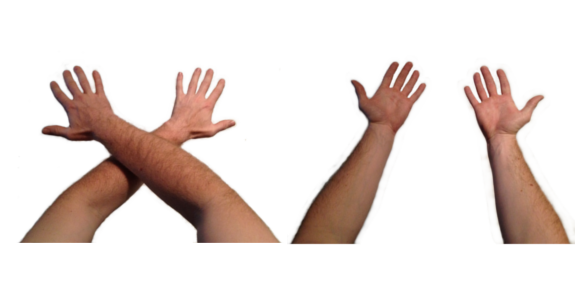
\includegraphics[width=0.5\textwidth]{figures/handAmbig}
\caption{Thumb position alone is not sufficient to disambiguate hands. Other data is required in the case of cross body reach.}
\label{fig:hand_cross}
\end{figure}

While it is possible to create a generic data fuser that merges incoming data from different sources into the same skeleton for most situations, it is not possible to create a fuser that will work for every possible system setup. For instance, the Leap Motion Controller cannot tell if the hand it is tracking is oriented palm up or palm down. This limitation means that its hand position will always be ambiguous since it cannot be sure which hand is being tracked when the user moves his hands into the the Leap’s tracking box while reaching across his body like in pose A in figure \ref{fig:hand_cross}. A second sensor is necessary if the application developer wishes to eliminate the ambiguity. In the case of the Jester sample application discussed in chapter \ref{chap:sample_app}, the PrimeSense Carmine is used to disambiguate hand position. The Carmine has long enough sensing range and a wide enough field of view to capture and track the user’s entire skeleton but does not sense wrist position as accurately as the LeapMotion Controller. A default data fusion class could easily assign a higher weight to the Leap’s wrist position and integrate the non-overlapping bones into the same skeleton. However, a true disambiguation requires the ability for the fuser to realize that the user is doing cross body reach pose A and reassign the false finger data that results from assuming the more natural pose B in figure \ref{fig:hand_cross}. Situations like this illustrate the necessity of modular and developer programmable data fusion units as well as the unfortunate reality that there cannot be a universal data fusion solution.

There are many different kinds of sensors that can be used to track different parts of the human body that all have different strengths and limitations. Most sensors have different APIs for retrieving skeletal tracking. In order for a sensor abstraction system like Jester to see wide adoption, input support for a large number of sensors and APIs is required. Since Jester is not backed by a large company and will not have full time developer support it is critical that third party developers can create and share sensor wrappers without requiring changes to the core of Jester. Unfortunately, abstraction alone is not sufficient to create a truly sensor agnostic system because an application may require data that the sensors present are not capable of providing; for example a system with only a Leap present cannot resolve the user’s head position. 

Jester’s flexibility requirements necessitate that Jester provides a sensor abstraction that allows developers to create thin wrappers for any skeletal tracking API that are distributable separately from the Jester core API as well as easily adaptable data fusion classes. This chapter will cover the core Jester functionality: the datapath, internal skeletal representation, and spatial transformation systems. It will also explain the sensor abstraction, data fusion, and data filtering architecture.

\section{Jester Core}\label{sec:jester_core}

Jester’s sensor wrappers and data fusion units need to be flexible in order to be useful. However, Jester’s core functionality and abstraction base classes should remain relatively constant in order to ensure backwards compatibility with older sensor wrapper and fusion implementations. If the abstraction interfaces are  designed correctly, the core should not need to be modified by developers. Therefore the Jester datapath, internal skeletal model, spatial transforms, and abstraction interfaces are kept separate from their implementations and are known as the Jester core. The Jester core is designed to be compiled into a library and does not need to be recompiled when new sensor wrappers or data fusion or filtering modules are created.

\subsection{Data Path}

Jester requires a data path that does not rely on sensors having any knowledge of the internal skeletal model or any other sensors that may present in order to allow sensor modules to be truly modular. So, there must be a black box style system for passing data from the sensor wrappers to the data fuser and then into the internal skeletal model. 

\begin{figure}[]
\centering
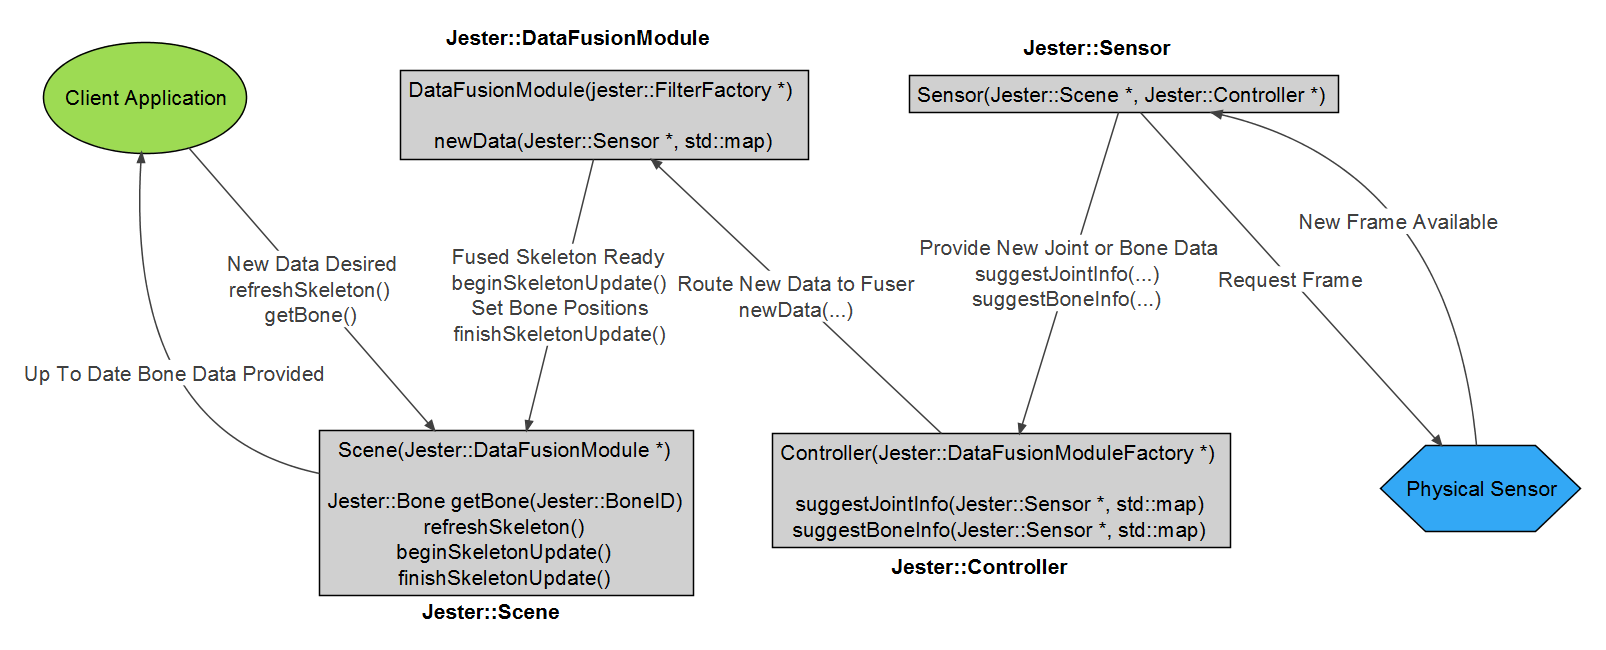
\includegraphics[width=1\textwidth]{figures/mainDataFlow}
\caption{The Jester core classes and dataflow paths.}
\label{fig:broad_datapath}
\end{figure}

The data path, illustrated in figure \ref{fig:broad_datapath}, centers around a controller class. The controller is constructed with a pointer to a data fusion class factory that is chosen or implemented by the application developer and is the center of a multi-step setup process depicted in figure \ref{fig:const_order} and described here. The Jester core comes with a data fusion implementation and factory that is adequate for straightforward fusion requirements; its design and implementation are discussed in section \ref{sec:fuser_des_impl}. When the controller is constructed using the constructor depicted in figure \ref{fig:broad_datapath}, it invokes the data fusion factory and then constructs an instance of the scene class with a pointer to the factory. The scene class is the root of the hierarchical skeletal model and is responsible for constructing and providing access to the bones that make up the skeleton. The scene class functionality is explained in section \ref{sec:scene_impl}. The controller then sets the newly created scene class to be the root space of the data fusion module in order to provide a common space in which to unite measurements and allow the fuser to cooperate with the scene to resolve race conditions discussed later. The controller, and therefore the scene and skeleton, must be constructed before individual sensors because sensors are a part of the scene graph along with the skeleton. The scene graph will be thoroughly explained in section \ref{sec:bone_hierarchy}, but, briefly, placing sensors in the scene graph allows sensors to be mounted to body parts and automatically handled by the space unification system discussed in section \ref{sec:bone_hierarchy}. 

\begin{figure}[]
\centering
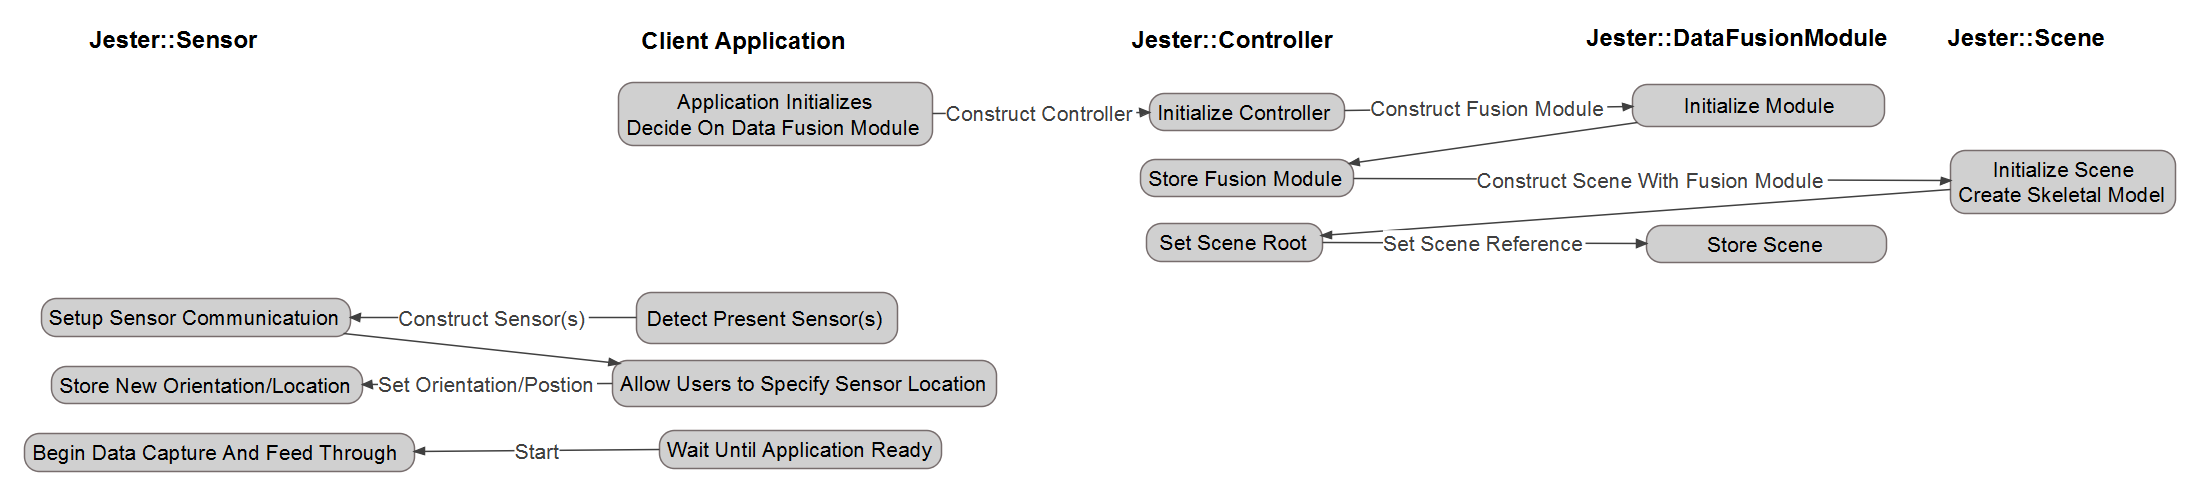
\includegraphics[width=1\textwidth]{figures/constructionOrder}
\caption{The Jester core construction order. Each column represents the task of that class or object. Vertical alignment denotes timing.}
\label{fig:const_order}
\end{figure}

Once the controller and scene are initialized, the application constructs the sensor classes for the sensors that are present in the system. Jester does not detect available sensors because there are simply too many different kinds and some setup specific manual configuration, discussed in section \ref{sec:sensor_wrappers}, is necessary. The sensor base class constructor requires pointers to the sensor’s scene graph parent and the controller. The scene graph parent pointer is necessary to provide a spatial context for the sensor measurements and will be discussed in sections \ref{sec:scene_impl}. The Jester controller provides a pair of functions called Controller::suggestBoneInfo(...) and Controller::suggestJointInfo(...) that allow the sensor class to asynchronously feed data into Jester when it arrives from the sensor API and without any knowledge of the timing issues, discussed in section \ref{sec:fuser_des_impl} that arise from having multiple sensors present in the same system.

When the Controller::suggestBoneInfo(...) or Controller::suggestJointInfo(...) are called the controller invokes the DataFusionModule::newData(...) function using the pointer to the data fusion module that was provided at the time of its construction with the same arguments that were received by the controller. The  data fusion module is responsible for storing the new skeletal data internally and fusing it asynchronously with data from other sensors in the system to form a complete skeletal model. The data storage and fusion process will be explained in section \ref{sec:fuser_des_impl}.

Once the sensor data has been fused into a cohesive skeletal model, the only remaining step is to provide access for applications. The controller provides a getter function to retrieve a pointer to the scene root class. The scene root is the parent of the skeleton and contains accessor methods to retrieve the individual bone positions. The process of initializing the Jester core and retrieving the skeleton for the first time requires less than 10 lines of code.

\subsection{Core Data Representation}

In computer graphics and animation the human skeleton is generally represented as a hierarchical model where each bone position depends on the position of the previous bone. Hierarchical modeling is a good analog to how the human skeleton actually behaves \cite{parent2012computer}. For example if a person swivels her upper arm, or humerus, at her shoulder but does not change her elbow or wrist angle the position of her hand still changes as illustrated in figure \ref{fig:arm_swivel}. Rather than marching down the chain of bones affected by the humerus and updating their 3D position every time there is a small change in parent position it is much more efficient to store each bones position relative to its parent. With relative positioning, parent position changes are automatically reflected when the child position is resolved.

\begin{figure}[]
\centering
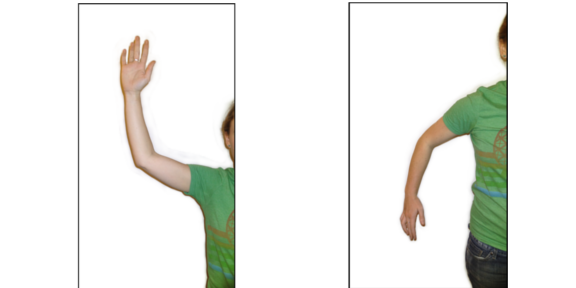
\includegraphics[width=1\textwidth]{figures/upDownSwivel}
\caption{The position of the hand changes greatly when the shoulder is swivelled, even if the elbow angle does not change.}
\label{fig:arm_swivel}
\end{figure}

Jester uses a spatial mathematics library called OpenGL Mathematics (GLM). GLM is a header only C++ library and so can be used on any system with a C++ compiler. It is designed to provide all of the functionality that a graphics application would need, and provides all of the quaternion, vector, and matrix operations needed for Jester. There are many solid math libraries, but GLM is commonly used in the graphics community because it is designed to mirror the GLSL API used in OpenGL programming \cite{glm}.

\subsubsection{Hierarchical Skeleton}\label{sec:bone_hierarchy}

In Jester, each bone stores a length, 3D start position in reference to the end of the parent, and an orientation as a quaternion with respect to the parent orientation. Each bone creates its own space where the bone runs down the positive Z axis. In order to take a point in one bone’s space and transform it to its parent’s space Jester creates a 4x4 matrix by translating an identity matrix by the bone’s starting position and then multiplying the new matrix by a rotation matrix derived from the bone orientation quaternion. The resulting matrix is known as the transform for the bone’s space and can translate any point from the bone’s space to its parent’s space. To transform a point from bone space all the way to world space, or the root space for the application, the 4x4 transforms for each bone in the hierarchy are multiplied to form one world transform. Similarly, the rotation of a bone in its parent’s space, and, by extension, world space, can be determined by multiplying the orientation quaternions together until the desired space is reached. The chaining of bone spaces can be visualized as seen in figure \ref{fig:joint_spaces}. Rendering a bone in OpenGL is as simple as rendering a cylindrical triangle mesh with a model matrix that is defined by scaling the bones world space transform by the whatever width the developer desires and the bones internally stored length.

\begin{figure}[]
\centering
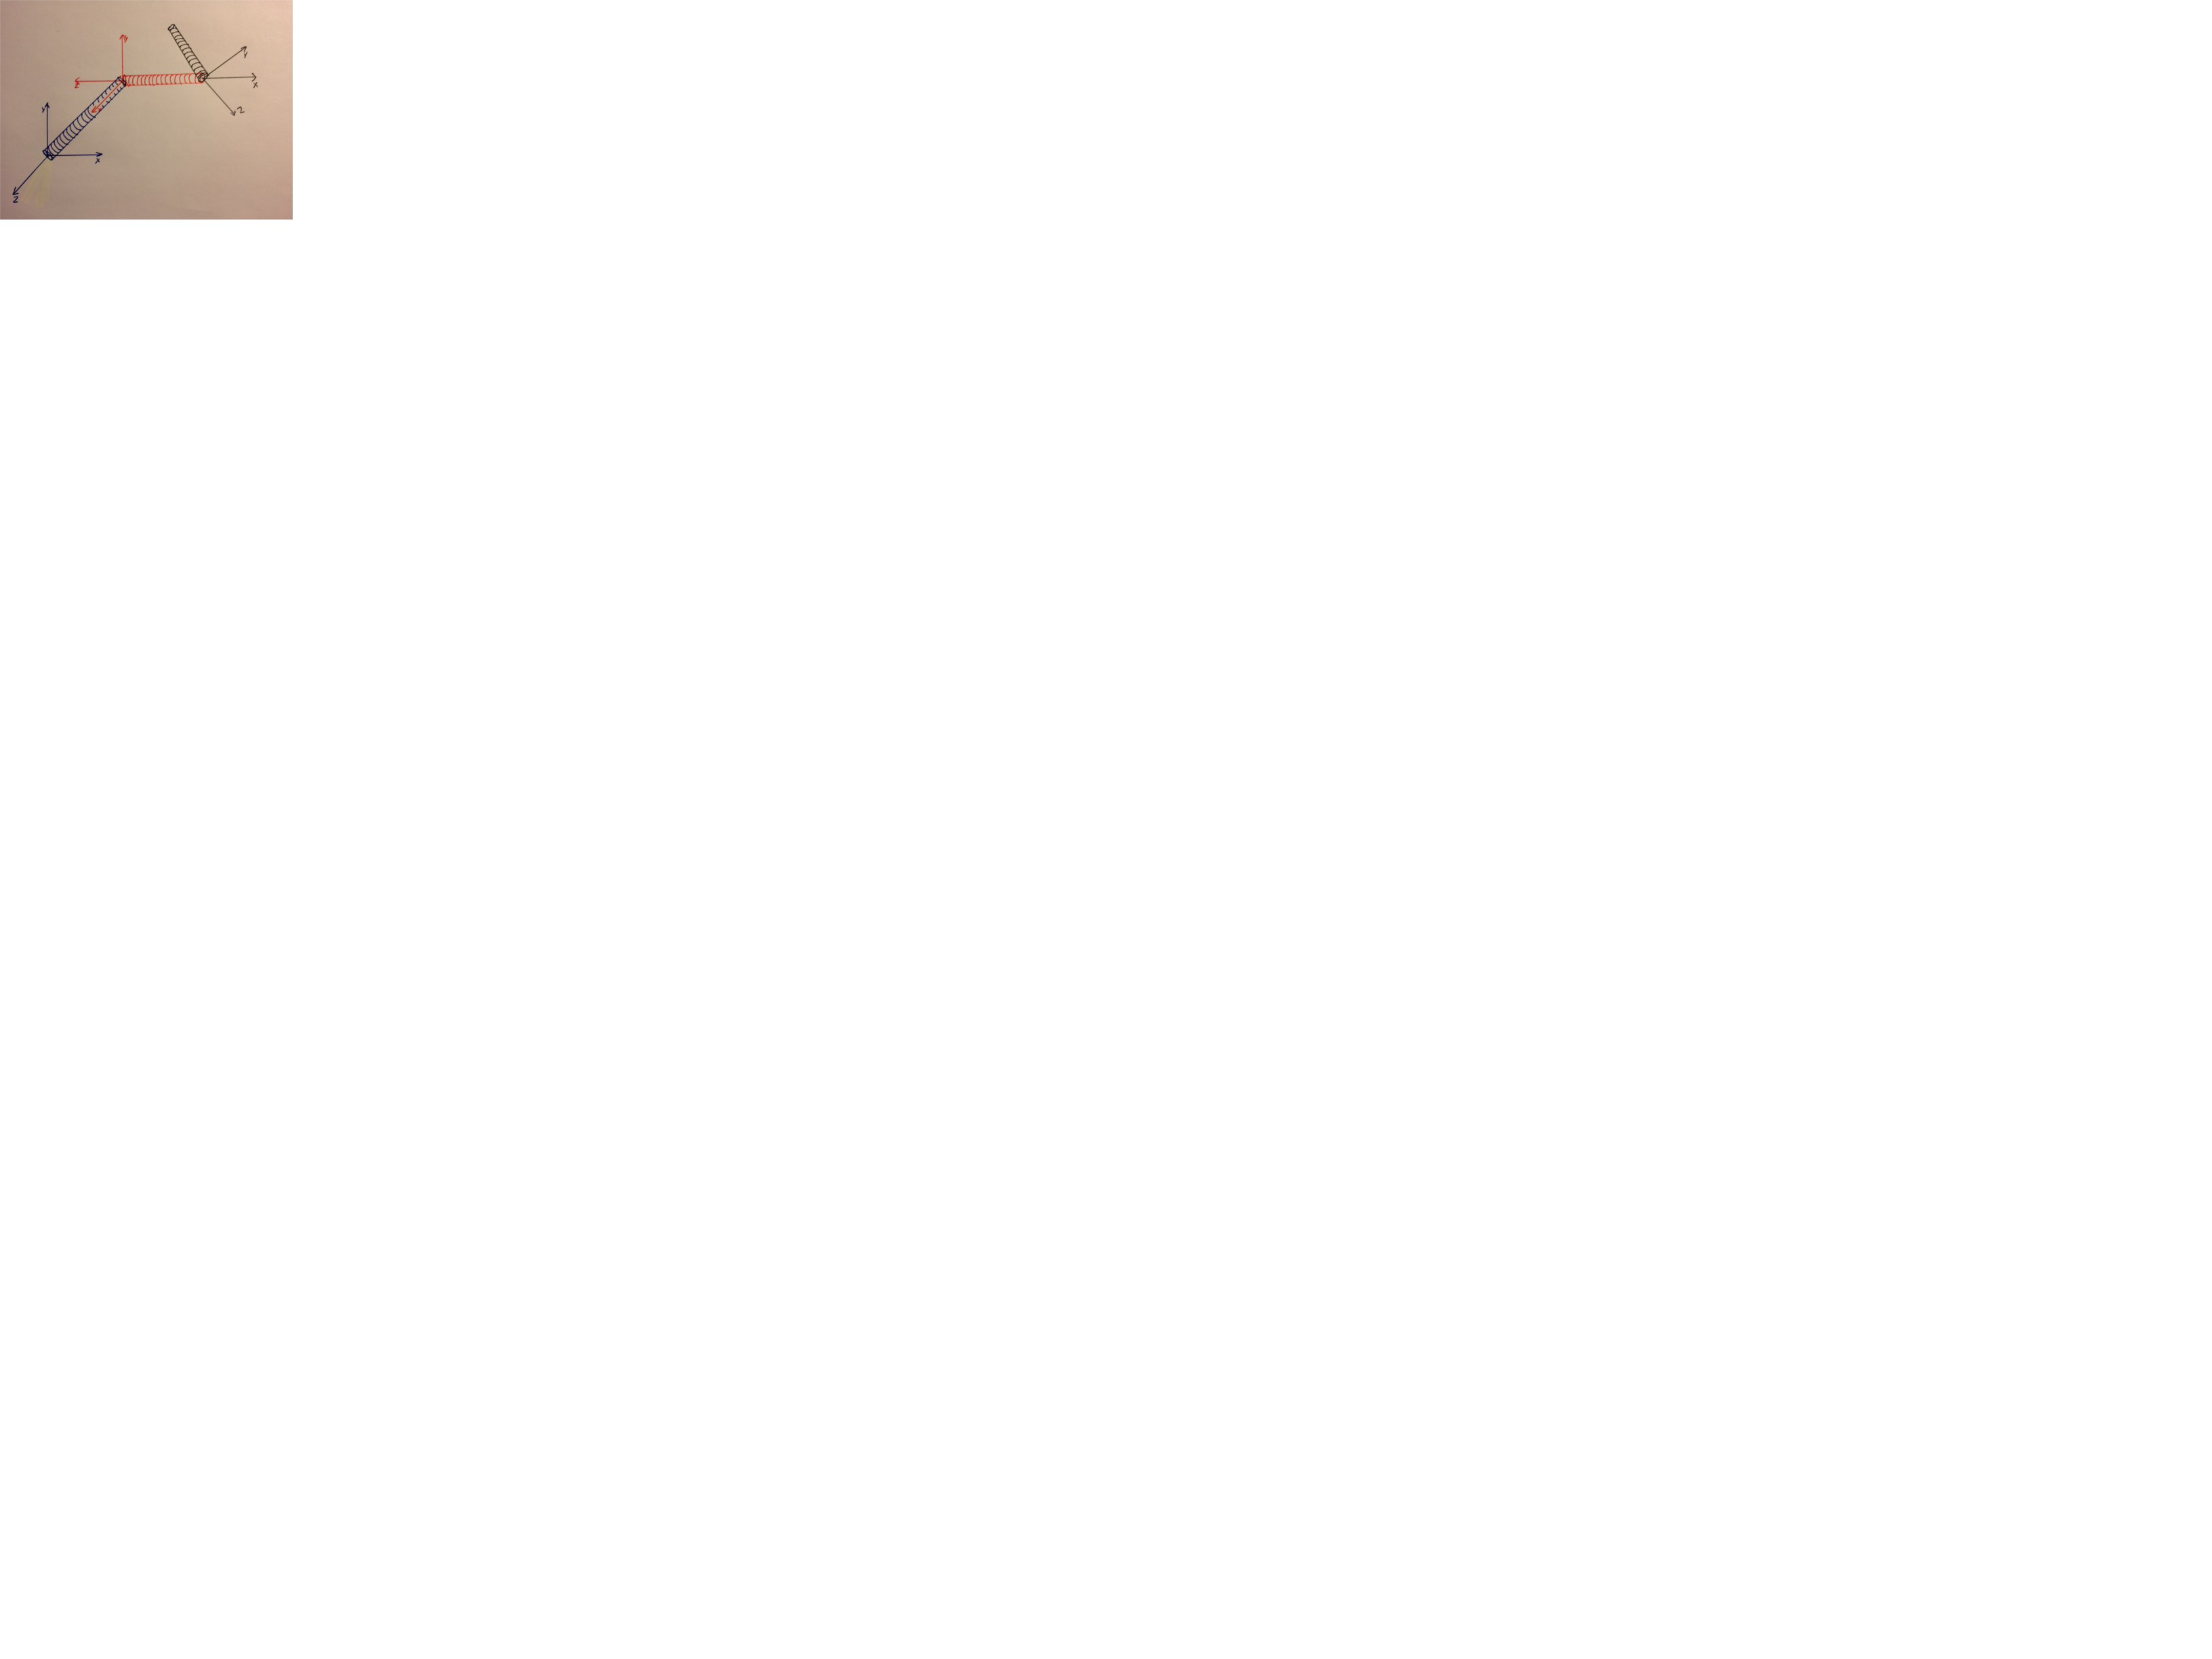
\includegraphics[width=.5\textwidth]{figures/spaceChain}
\caption{Each bone in the kinematic chain has its own basis space defined by its orientation relative to its parent.}
\label{fig:joint_spaces}
\end{figure}

Jester's reduced bone set maps well to the bones that can be tracked by current skeletal sensors. Figure \ref{fig:skeleton} shows the bones that have been selected. The Jester skeleton is hierarchically based on a fictional "root bone" that is is placed at the midpoint of the pelvis. A fictional bone is used because there is no centrally placed bone in the human torso that does not have other bones attached at both ends. Having children bones only placed at one end of the root allows the system to have one consistent pivot point and simplify the conceptual complexity. The head was not selected for the root because placing the head at the root would essentially rotate the entire body as the head is turned, which is not consistent with what happens in reality.

\begin{figure}[]
\centering
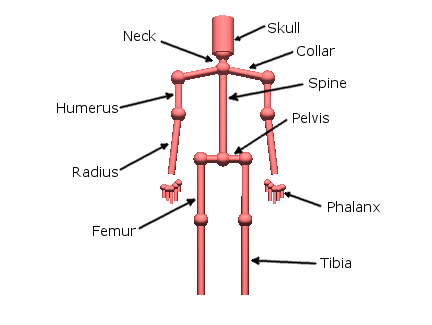
\includegraphics[width=.75\textwidth]{figures/boneLabels}
\caption{The Jester skeleton. Mirrored bones are stored as bone\_L or bone\_R. Phalanx are numbered 1-5 with 1 being the thumb.}
\label{fig:skeleton}
\end{figure}

The skeletal bones themselves compose just one part of the scene graph provided by Jester. All components of the scene graph are children of the parent class Jester::SceneGraphNode. Jester::SceneGraphNode provides the base functionality for calculating the local and world position, orientation, and transform. It also tracks the node’s children and parent. Providing a generic base class for the Jester scene graph allows developers to easily incorporate the Jester scene graph into their application rather than building a custom one. If developers want to add things besides sensors to the scene graph they just have to extend the Jester::SceneGraphNode superclass. The built in scene graph inheritance is depicted in figure \ref{fig:scene_graph_inh}.

\begin{figure}[]
\centering
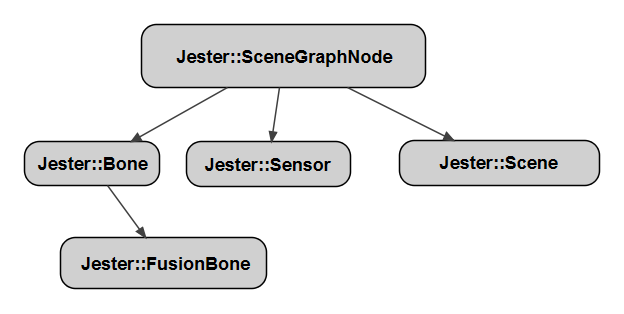
\includegraphics[width=.75\textwidth]{figures/sceneInh}
\caption{Jester's scene graph inheritance hierarchy.}
\label{fig:scene_graph_inh}
\end{figure}

Jester’s abstract Sensor class is a subclass of Jester::SceneGraphNode. Placing Sensors in the scene graph greatly simplifies the process of merging the data from different sensors. Most sensors provide bone data with respect to their space; meaning that if the sensor is moved but the sensed bone is not the sensor will think that the bone is what moved. Similarly, two identical sensors placed side by side will track the same bones but report slightly different positions. Most sensors are statically mounted on tabletops or walls, but it makes sense to mount some sensors on the human skeleton itself. For instance, a user could mount a hand tracking sensor on her head mounted display so that she could turn to look at virtual objects and then interact with them naturally without worrying about the sensor field of view like she would if it was placed on a desk. Including sensors in the scene graph makes it possible to simply use the world space transform provided by Jester::SceneGraphNode to move sensed bone positions into Jester’s world space. 

\subsubsection{Scene Root}\label{sec:scene_impl}

The root of the Jester scene graph is the Jester::Scene class. It provides the base space for all scene graph nodes as well as accessor functionality for the bones that make up the skeleton. While the Jester::SceneGraphNode class provides access to an std::iterator that makes it possible to traverse the skeleton by starting at the scene root and recursively iterating over all of the children of each node, that process would be unnecessarily cumbersome if the user just wants to access a specific bone. So, the scene class provides a function called Scene::getBone(...) that takes the ID of the desired bone and returns a pointer to the correct bone object.

\begin{figure}[h]
\centering
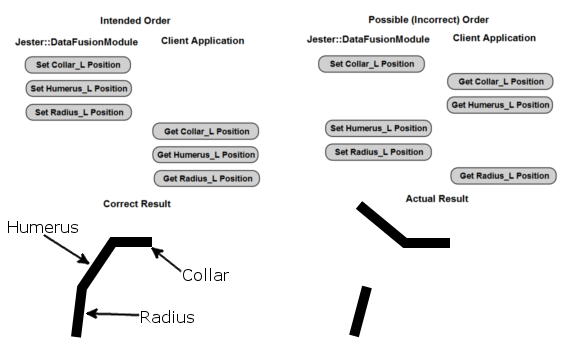
\includegraphics[width=1\textwidth]{figures/dataRace}
\caption{Not synchronizing the process of updating and setting the skeleton can result in wildly incorrect skeletal data.}
\label{fig:data_race}
\end{figure}

The scene class also cooperates with the data fuser to provide a consistent and up to date skeleton. If the data fuser actively modified the same bone objects that are in the scene, there is a possibility that applications could render an inconsistent skeleton. Since both the data fuser and applications access the skeleton in pieces and are operating concurrently in separate threads, there is an inherent race condition illustrated in figure \ref{fig:data_race}. If a single threaded client application is attempting to render the current position of the user’s right arm, it will access the position of the humerus, then the position of the radius, and then the fingers. If the data fuser updates the position of the arm before the client accesses the radius but after the position of the humerus, the bones could be rendered disconnected from each other.

Jester solves the inconsistency problem by using a double buffering approach shown in figure \ref{fig:double_buffer}. The scene holds two sets of skeletons; one for the data fuser to update and one for the client application to read. Both skeletons are updated whenever the SceneGraphNode::addChild(...) or SceneGraphNode::removeChild(...) functions are called. The data fuser notifies the scene when it is about to modify the skeleton by calling Scene::beginSkeletonUpdate() and when it is done by calling Scene::finishSkeletonUpdate(). Locking the fusion skeleton tells the scene that it should not swap the skeletons while the data fuser is in the process of changing data. Client applications call Scene::refreshSkeleton() when they want the most up to date complete skeleton. Scene::refreshSkeleton() checks if the skeleton is currently being updated. If it is, then the client thread is blocked until the data fuser is done updating or a short timeout expires. The timeout allows the client application to not stall for long if the data fuser is hanging in order to help ensure that the client UI does not lock. Once the block is released without timeout or if the skeleton was not currently being updated, the scene enables a lock in Scene::beginSkeletonUpdate() to make the fuser wait, swaps the two skeletons so that the client application gets the most up to date data and the data fuser gets a new skeleton to modify, and disables the lock in Scene::beginSkeltonUpdate() to allow the fuser to continue. Double buffering in this manner allows Jester to support multithreaded data fusion while preventing the possibility of providing an inconsistent skeleton.

\begin{figure}[]
\centering
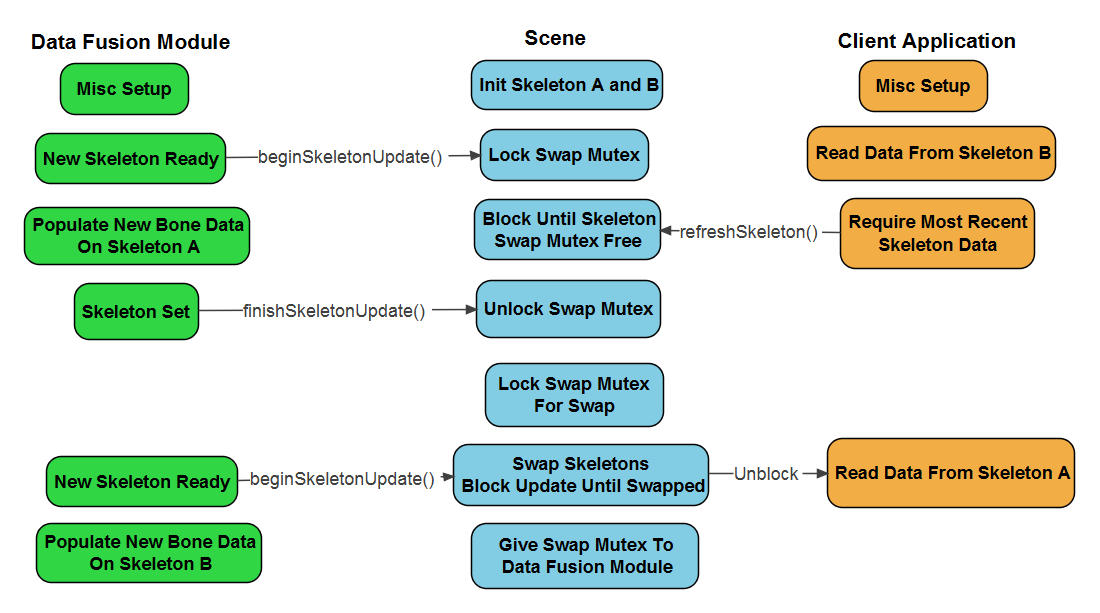
\includegraphics[width=1\textwidth]{figures/doubleBuffer}
\caption{Double buffering the skeleton prevents the race condition from figure \ref{fig:data_race}.}
\label{fig:double_buffer}
\end{figure}

\subsection{Joints}

The position of many bones in the human body can be determined using the joints that they connect. For example, the position of the radius can be completely determined using the position of the wrist and elbow joints. Many sensors, like the PrimeSense Carmine, report skeletal position using joints instead of bones. So, the Jester framework accepts skeletal data as bone position or joint position. Bone position maps directly into the Jester skeleton, but joint data requires some special handling.

Jester has convenience functions to handle the resolution of bone position from the position of two joints. The Jester::Bone class provides enumerations for all of the bones that are supported by Jester and all of the joints that can be used to define those bones as well as a map that takes a bone ID and returns the pair of joint IDs that defines it. The Jester fusion module superclass, Jester::DataFusionModule, provides a function called getBonesFromJoints(...) that resolves bone positions by looping through the bones that are supported by Jester and checking to see if the joints mapped to each bone were provided. If both Joints were provided, the function simply sets the bone to start at the start joint and terminate at the end joint. Since not all sensors provide information about all of the joints supported by Jester, it is possible that a bone could be missing one or both joints. It is useful to provide default joint positions that can be used if joints are missing. For example, if a system only uses a LeapMotion Controller, it will be able to track the user’s wrist position but not his elbow. Jester can still create a skeleton with just the wrist positions by using the default joint positions for the unmapped joints. Assuming default joint position frequently results in distorted bone lengths as shown in figure \ref{fig:distorted_bones}, but it is not possible to infer joint position without a true inverse kinematics engine. We have decided that, for Jester, it is better to provide a possibly inaccurate skeleton than to force users to have sensors tracking every joint in order to get any data.

\begin{figure}[]
\centering
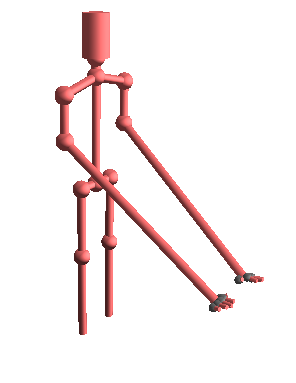
\includegraphics[width=.3\textwidth]{figures/distortedBones}
\caption{Using data from a sensor that only provides data from one joint that defines a bone results in distorted bones.}
\label{fig:distorted_bones}
\end{figure}

\section{Plugin Architecture}

The Jester core provides the functionality that is not sensor or system setup dependent. The previous section touched on the design of the sensor wrapper and data fusion classes in order to explain the Jester data flow. This section will detail the design of the modular components of Jester. Sensor API interaction, sensor fusion, and data filtering are all parts of the skeletal data input process that may need to change widely for different system implementations. So, the supporting base classes are designed to provide the basics while allowing developers to easily create custom modules.

\subsection{Sensor Wrappers}\label{sec:sensor_wrappers}

The design of the Jester sensor wrappers is probably the simplest of any class in the entire system. Developers will frequently have to be able to create their own custom wrappers for different sensor APIs because there are so many, and the core concept of Jester is to be able to support as many different sensors as possible. Due to the flexibility requirements, the specific implementation of each sensor wrapper internals is completely left to the developer. The only requirements are that the developer's sensor class be a subclass of Jester::Sensor and that it delivers data to the Jester skeleton by calling Controller::suggestJointInfo(...). 

Jester::Sensor takes Jester::SceneGraphNode and Jester::Controller pointers. The Jester::SceneGraphNode is necessary because Jester::Sensor is a subclass of Jester::SceneGraphNode and designed to be placed into the scene graph. Providing a pointer to the graph node's parent at the time of construction allows the Jester core to automatically add the new sensor to its scene graph parent's list of children. The controller pointer is not used by the Sensor superclass, but the sensor wrapper implementation will need it to pass skeletal data to the Jester core. Requiring the Jester::Controller pointer as a part of the superclass implementation makes the controller requirement apparent and attempts to simplify the process of creating sensor implementations. 

Unsurprisingly, different skeletal tracking APIs require different query methods. Some allow developers to register a callback function to handle new data. Others need to be queried continuously. Whatever the data fetching method is used will be responsible for pulling skeletal bone or joint data from the device API and mapping it to the joints or bones that are supplied by the Jester API. If there is not a one to one mapping, the sensor wrapper implementation is responsible for either disregarding the data if the bone or joint has no close analogue or translating the data if it is similar. For example, the LeapMotion API senses palm position, and the closest thing in Jester is the wrist joint. Since the LeapMotion API provides a vector for the direction the hand is pointing, a developer can simply translate the palm position a small distance in the opposite direction of the hand vector to estimate wrist position. The specific implementation details of two example sensor wrappers will be discussed in the next chapter.

The client program is responsible for either detecting the sensors present in the system or providing the user with a way of selecting their system setup. Once the client has constructed the Jester controller and the correct sensor wrappers for their system they must specify the position and orientation of the sensors with respect to its parent object in the scene graph. If the sensor is placed on an immovable surface then its parent should be the scene root, and if it is mounted to a body part, like the head, then its parent should be the bone that approximates that part. The Jester::Sensor superclass exposes functions for setting the orientation and position of the sensor. The position of the scene root center is arbitrary, so it is entirely up to the application developer. As long as the sensor positions are set relative to the same 3D point and orientation, they will form a coherent skeleton. The initialization code for a specific demo application will be discussed in section \ref{sec:app_impl}, and the implementation of two sensor wrappers in sections \ref{sec:leap_impl} and \ref{sec:carmine_impl}.
	
\subsection{Sensor Fusion}\label{sec:fuser_des_impl}

Sensor fusion requirements can vary widely depending on the type of sensors present in the system. So, the Jester sensor fusion module superclass is designed to provide a base level fusion implementation that can used as is, modified slightly to fit small differences in system needs, or even completely replaced. This section will explain the design of the base implementation and the methods for making small modifications; large modifications are too diverse to enumerate and anything can be replaced since all of the Jester::SensorFusionModule methods are abstract.

The default sensor fusion module requires application developers to tell it which sensors to expect data from by calling the SensorFusionModule::registerSensor(...) function. registerSensor(...) takes the Jester::Sensor pointer to one of the sensors that is present in the system and a map that maps either a bone ID or a joint ID to a weighting scaling value. The weighting scaling value is used to decide how much to trust measurements from that sensor about that bone or joint and will be explained in more detail shortly. The data fuser is ready to handle new bone or joint position data once all of the sensors have been registered.

Jester sensor wrappers operate in separate threads, so the sensor fusion module will be responsible for handling the inherent synchronization problems that occur when different parts of the skeleton arrive at different times shown earlier in figure \ref{fig:data_race}. This becomes especially important when multiple sensors are sending data about the same bone. The SensorFusionModule::newData(...) function is called asynchronously, so it requests a lock on a skeleton modification mutex before attempting to merge the new data with the internal skeletal model. It also keeps a history of the sensor readings as a series of independent skeletons, or "skeleton frames", to help match the data between sensors temporally. Skeleton frames are their operation are illustrated in figure \ref{fig:skeleton_frames}. The fuser runs a thread that is responsible for updating the scene's skeleton. At a set interval it examines the skeleton frame history to get the best current skeleton. If the current frame does not have data about a specific bone, it looks backwards in time a user-configurable number of frames to find the most recent known position. If it finds position data, it uses it to build the skeleton, but if there is no data within the set number of frames it uses the default bone position. After setting the skeleton, it advances the history to the next frame. 

SendorFusionModule::newData(...) accepts skeletal information as either bones or joints and Jester operates internally using bones; both data input processes are illustrated in figure \ref{fig:new_data_flow}. So, joints are transformed into bone data using the bone to joint lookup map discussed in the datapath section. If there is a filtering module present the fuser sends the new bone to the filter and then replaces the sensed position with the one given by the filter. The fuser then checks if there is any information about the new bones already in the current skeletal frame. If the data has not been set yet or is from the same sensor, the new bone position is inserted. If there is data from a different sensor, then the new position is fused by interpolating between the competing bone start positions and quaternions using a weighting equating that is a combination of the confidence supplied by the sensor reading and the scaling value for that bone [math and explain]. The frame is advanced if all of the sensors have contributed to the current frame once the data is inserted and fused. 

The length of the skeleton frame history, the number of frames to go back in time when setting the scene skeleton, and the amount of time before the frame is auto-advanced are all easily configurable to match the real time needs of the system. Frequent updates are more demanding, but provide a more current system if the sensors can keep up. The new data handling process is all handled with virtual methods, so data fusion implementations can easily change the data handling for some bones while invoking the default fusion functions with others. An example of small modifications to the fusion system is given in section \ref{sec:fuser_impl}.
	
\subsection{Data Filtering}

Different data filtering methods require very different implementation details so the Jester data filtering module provides little functionality other than a public interface for invoking the filter so that filters are somewhat easily swappable. The human skeleton has more many degrees of freedom than the filtering methods investigated for this thesis can reasonably handle so we assume that there will be a filter for each bone in the body. The Jester::DataFilter base class has an abstract virtual functions for initializing the filter, DataFilter::init(), and updating the filter with the current sensed position of the bone, DataFilter::update(...). The init function is responsible for doing any setup that the filter requires and the update function passes in the best known position of the bone. The filter is responsible for updating its internal algorithm with the new data and returning the filtered bone position. A sample particle filter is implemented in section \ref{sec:filer_impl}.


\chapter{Sample Implementation}\label{chap:sample_app}

A sample toy application has been created to validate the Jester sensor and data fusion abstraction framework. It uses the LeapMotion Controller and the PrimeSense Carmine to allow the user to either deflect or delete balls with their character's hands as they fall from the sky. These two sensors were selected because they provide an overlap of data about the users skeleton as described at the beginning of Chapter \ref{chap:api_des}. Properly fusing the data in this system will require a small modification of the default data fusion module in order to handle the hand orientation ambiguity. This section will discuss the implementation of the required sensor wrappers, data fusion modifications, and a sample filtering algorithm.

\section{Sensor Wrappers}

The LeapMotion Controller and the PrimeSense Carmine are manufactured by different companies and use completely different skeletal APIs. So, each needs its own wrapper implementation. Ideally, there would be a support community of VR enthusiasts that would create sensor wrappers for new hardware and provide them to others. However, that will not exist initially and the process of creating wrappers must be demonstrably simple. This section will cover the process for creating wrappers for the LeapMotion Controller and the PrimeSense Carmine.

\subsection{LeapMotion Controller}\label{sec:leap_impl}

The LeapMotion Controller is designed for hand and finger tracking and has a relatively short range and narrow field of view, but is capable of tracking with high precision. LeapMotion's API provides an interface for registering a callback function that is triggered when there is new information about the hands visible. The callback is called with a reference to the current captured frame. The frame provides an accessor to get a list of all of the hands that the Controller can resolve in the current frame. The Controller can track as many hands as can cleanly fit in its field of view. Each hand has an ID that is unique to that hand. However, if the Controller loses tracking of a hand it will assign it a new ID. Similarly, each hand has a list of fingers; each with a unique ID. The IDs are assigned randomly and the API does not provide a guess about which finger is which. So, it is left to the developer to best decide how to resolve hand and finger identity.

This thesis resolves right and left hand position using a set of assumptions that must be followed for correct system behavior:

\begin{enumerate}
	\item There will never be more than 2 hands in the Controller's tracking space.
	\item If only one hand is inserted into the tracking space it is the left hand if it is to the left of the center of the Controller, and the right if it is to the right. This only holds true when the hand is first seen. Once that hand's ID is assigned it can move to either side of the Controller freely.
	\item If one hand is being tracked, the next hand that the Controller tracks is assigned to be the other.
\end{enumerate}

These rules have been experimentally determined to be effective most of the time. However, it is possible for the Controller to become confused and swap the hands it is tracking. The hands can be reset by withdrawing them from the tracking space, waiting a second, and then reinserting.

\begin{figure}[]
\centering
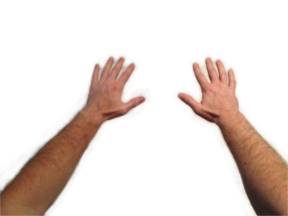
\includegraphics[width=0.5\textwidth]{figures/handsStraight}
\caption{The user's hands must be placed in front of the LeapMotion Controller with palms down and fingers spread in order to calibrate.}
\label{fig:hand_default}
\end{figure}

Finger tracking in the Leap is a bit more complex. Using the X-axis position of the fingers is unreliable in situations where the hands are rotated so that the fingers are pointing outward. The Controller API attempts to provide a vector that points along the hand direction, but it is unreliable. This thesis's implementation uses a calibration pose to solve the finger ambiguity issue. The wrapper waits until all five fingers are visible on the hand, and then assumes that the thumb is the inside finger along the X-axis and the rest of the fingers are placed normally with respect to that orientation as shown in Figure \ref{fig:hand_default}. It then retrieves the length of each finger from the LeapMotion API and assigns it to that hand for the rest of that hand IDs life. Next, it gets the finger IDs from the API and assigns them in the same manner. Whenever a finger ID is lost, the wrapper stops reporting information about that finger. When an unknown finger ID is attached to the hand, the wrapper finds the finger on the hand that is not currently being tracked and has the closest length to the new finger. The new finger's ID is then assigned to that finger. This process is detailed in Figure \ref{fig:finger_matching}. 

\begin{figure}[]
\centering
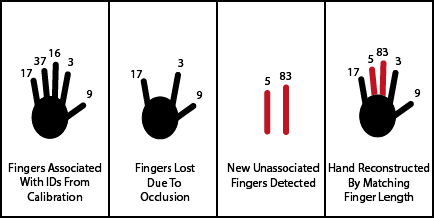
\includegraphics[width=.75\textwidth]{figures/fingerAssociation}
\caption{Finger IDs frequently become lost and must be reacquired using the calibrated length.}
\label{fig:finger_matching}
\end{figure}

Once the wrapper has calibrated finger length it begins to provide data about finger position. The LeapMotion Controller tracks finger tip position and orientation. Jester stores finger position using the knuckle joint and an imaginary joint placed at the end of the finger. The wrapper converts Controller finger data to Jester finger data by using the tip position as the imaginary end joint and estimating the position of the knuckle joint by moving backwards along the tip vector by the length of the finger.

The wrapper processes all of the hand and finger data that it can glean from the LeapMotion API on each invocation of the new frame callback. Once it has the LeapMotion objects for hands and fingers mapped, it translates the positions from LeapMotion points into GLM points and calls the controller's suggestJointInfo(...) method to pass it into the data fuser.

\subsection{PrimeSense Carmine}\label{sec:carmine_impl}

The PrimeSense Carmine is designed for full body tracking and has both a longer range and wider field of view than the LeapMotion Controller. It uses a skeletal tracking API called NiTE that was designed for the Carmine by PrimeSense. NiTE is capable of tracking all of the Jester bones that the LeapMotion Controller is not. There is also a very close to 1:1 mapping from the joints that are tracked by NiTE and the Jester joints. The Carmine wrapper only has to infer the position of the imaginary joint at the top of the head to generate head orientation and the position of the root bone, since it is not actually present on a skeleton.

The wrapper is implemented by setting up a polling thread that is launched when the Carmine wrapper is started. The thread simply polls the Carmine every 100ms to get new frame data. It assumes that the first skeleton present, since the Carmine can track multiple skeletons, is the relevant skeleton and waits until NiTE recognizes a full lock on its joint positions. Once a full lock has been achieved it converts the NiTE joints into GLM joints, assumes the head is always pointing up and that the root bone is at the midpoint between the two hip joints, and calls the controller's suggestJointInfo(...) method to feed the skeleton to the data fuser.

\section{Fusion Implementation}\label{sec:fuser_impl}

The data fusion requirements for the sample application are very close to being in line with the default functionality. There just needs to be a method for disambiguating the hand orientation from the LeapMotion Controller. So, the sample data fuser simply extends the default fuser and overrides the DataFusionModule::newData(...) function. The new implementation simply checks if the wrist joints are known in the current skeletal frame. If they are, then it checks if the incoming wrist joints would be closer to the existing positions if the hands were swapped like in Figure \ref{fig:hand_swap}. If the change in difference is larger than a threshold the fuser assumes that the hands need to be swapped. If the incoming data is from the LeapMotion controller, then it creates a new map where the hands and fingers are swapped and then invokes the superclass's newData(...) function with the new map. In the case where the Leap's finger data has already been placed in the current skeletal frame, the data in the frame is swapped and then the superclass's newData(...) function is called with the unchanged map. This small set of modifications to the base fuser class show that small system modifications are easy in situations where a close to default behavior is desired.

\begin{figure}[]
\centering
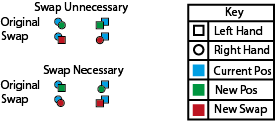
\includegraphics[width=0.5\textwidth]{figures/handSwap}
\caption{Hand position, represented as shapes, sometimes needs to be swapped due to data ambiguity.}
\label{fig:hand_swap}
\end{figure}

\section{Data Filtering}

The LeapMotion Controller provides very stable data, but the PrimeSense Carmine is prone to having joint positions suddenly "jump" from their correct location to a wildly incorrect position and then reset. So, the system stability can seriously benefit from filtering. This thesis implements a sample particle filter to attempt to reduce the system noise.

\subsection{Double Exponential Filter}\label{sec:filter_impl}\label{sec:double_exp}

A double filter was selected because it is good for applications where a system dynamics model is difficult or impossible to create as discussed in Section \ref{sec:filter_back}. Double exponential filters are extremely straightforward. The implemented filter simply stores the last filtered start and end points and their trends as glm::vec3s. When the update function is called with the new bone position, the orientation quaternion is used to calculate the bone end point because filtering the orientation directly was not possible using the filter equation. The start point and end point of the bone are filtered separately and then recombined to give a filtered start point and orientation quaternion. The newly filtered data is then returned from the update function.

\section{Sample Application}\label{sec:app_impl}

The sample application of Jester is mainly designed as a toy to prove that the concept of a sensor abstraction and data fusion framework can be useful. It is only vaguely useful and is only designed to showcase the cooperation between the PrimeSense Carmine and the LeapMotion Controller. Balls slowly fall from the ceiling and can either be deflected away or deleted on contact depending on if the user's hand is open or closed. A huge bulk of the code is devoted to handling mouse events, setting up OpenGL, and the simple physics engine. The implementation of all of these tools is outside the scope of this thesis. Jester's setup and query steps can be represented in the following steps that map 1:1 to code:

\begin{enumerate}
  \item Construct Jester Controller with Data Fuser Factory
  \item Construct Sensor object
  \item Set sensor orientation
  \item Set sensor position
  \item Add sensor to fuser
  \item Repeat 2-5 for each sensor
  \item Start sensors
  \item Get the Scene object from the Controller
  \item Call Scene::refreshSkeleton()
  \item Query Scene for bone position to draw skeleton
\end{enumerate}

The fact that so little of the application code is dealing with sensors and raw sensor data is a signal of the value of the Jester abstraction framework.


\chapter{Results}
\section{Jester Core Performance}
\section{Data Fuser Performance}
\section{Application Performance}

\chapter{Conclusion}
\chapter{Future Work}
\section{Inverse Kinematics}
\section{Joint Probabilities}

% ------------- End main chapters ----------------------

\clearpage
\bibliographystyle{plain}
\bibliography{Bibliography}

%\begin{appendix}
%%\addcontentsline{toc}{chapter}{\appendixnamelower}
%\include{Appendix}
%\end{appendix}

\end{document}